\chapter{Visual Perception}
The detection and recognition of the surgical tools and other objects of the simulation scene is the topic of this chapter. For complexity reduction we assume in the simulation that the surgical tools are blue and the mounting dock, where the tools will be placed, is green. These assumptions make the scene and object recognition much easier without the need of more advanced image  processing and/or machine learning recognition algorithms.\\

The used \textbf{Camera setup} has the following parameters:
\begin{itemize}
\item 2 HD RGB cameras with resolution $1280 \times 720$
\item near clipping plane: 0.02
\item far clipping plane: 300 
\item horizontal FoV (field of view): 1.396
\item update rate: 30~FpS
\end{itemize}

\section{Laparoscopic tool detection}
\label{laparoscopic-tool-detection}

In order to detect the shape of the tool there are some standard steps that need to be executed. After having loaded the input image we convert it to grayscale, so that we can work on only one channel. Next step is 
to remove the unwanted noise. In this thesis we only assume that the video frames have only Additive White Gaussian Noise (AWGN). To remove some of the noise we use a moving average filter (the filter is also known as a kernel), which is convoluted around the whole image. The filter that was used is the $
h = \frac{1}{9} \begin{bmatrix}
1 & 1 & 1 \\
1 & 1 & 1 \\
1 & 1 & 1 \\
\end{bmatrix}
$.~
The filtered image is the result of the convolution of the image with the filter and is calculated as 
$
g(i,j) = \sum_{k,l=-1}^1 f(i+k,j+l)h(k,l),~
$
where $g(\cdot, \cdot)$ is the output image and $f(\cdot, \cdot)$ is the input image.

After the noise is removed the image is transformed into a binary one by setting a threshold, below which the pixels will be black and the rest will be white. The conversion to this binary format, simplifies the extraction of the boundaries of the black shapes, which will corresopnd to the boundaries of the objects of the initial image.

\begin{comment}
  \section{Stereoscopic vision}
  \label{stereoscopic-vision}
  
  \begin{center}
  \begin{figure}[H]
  \centering
  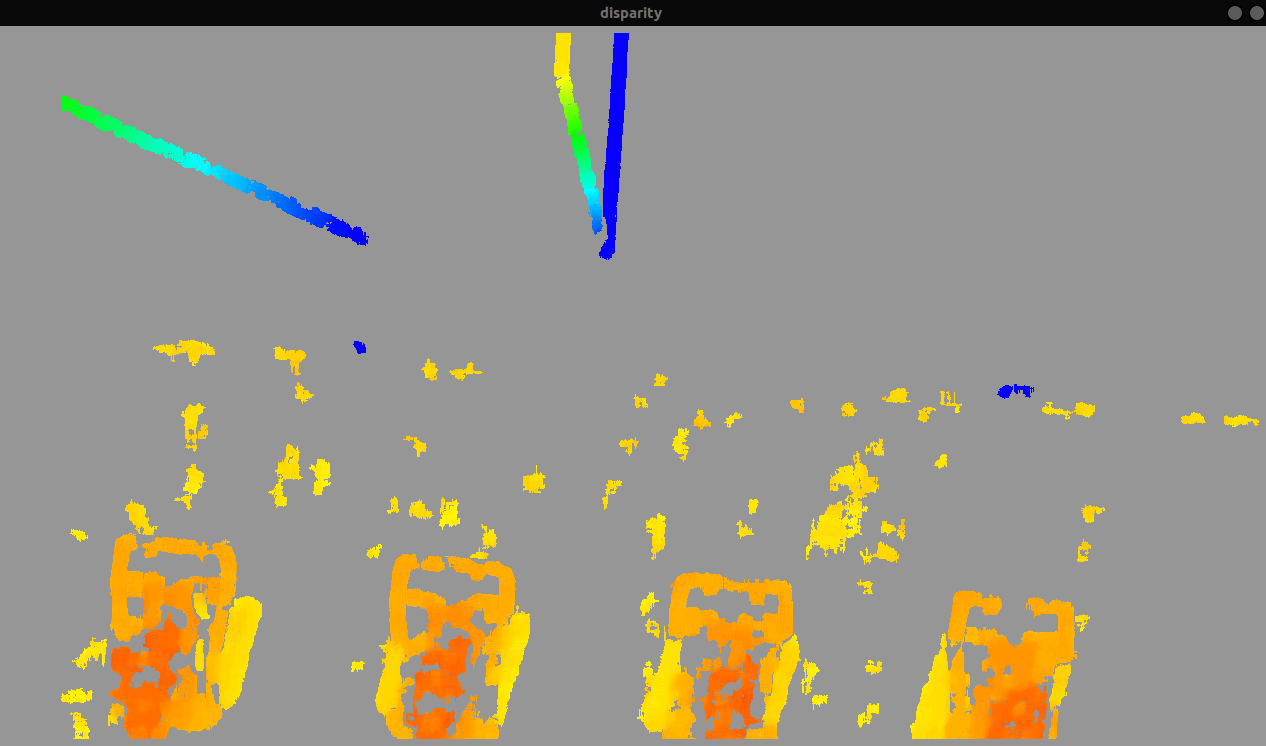
\includegraphics[width=12cm]{images/disparity.png}\\
  \caption{Disparity image calculated from the 2 cameras}
  \end{figure}
  \end{center}
  
  \begin{center}
  \begin{figure}[H]
  \centering
  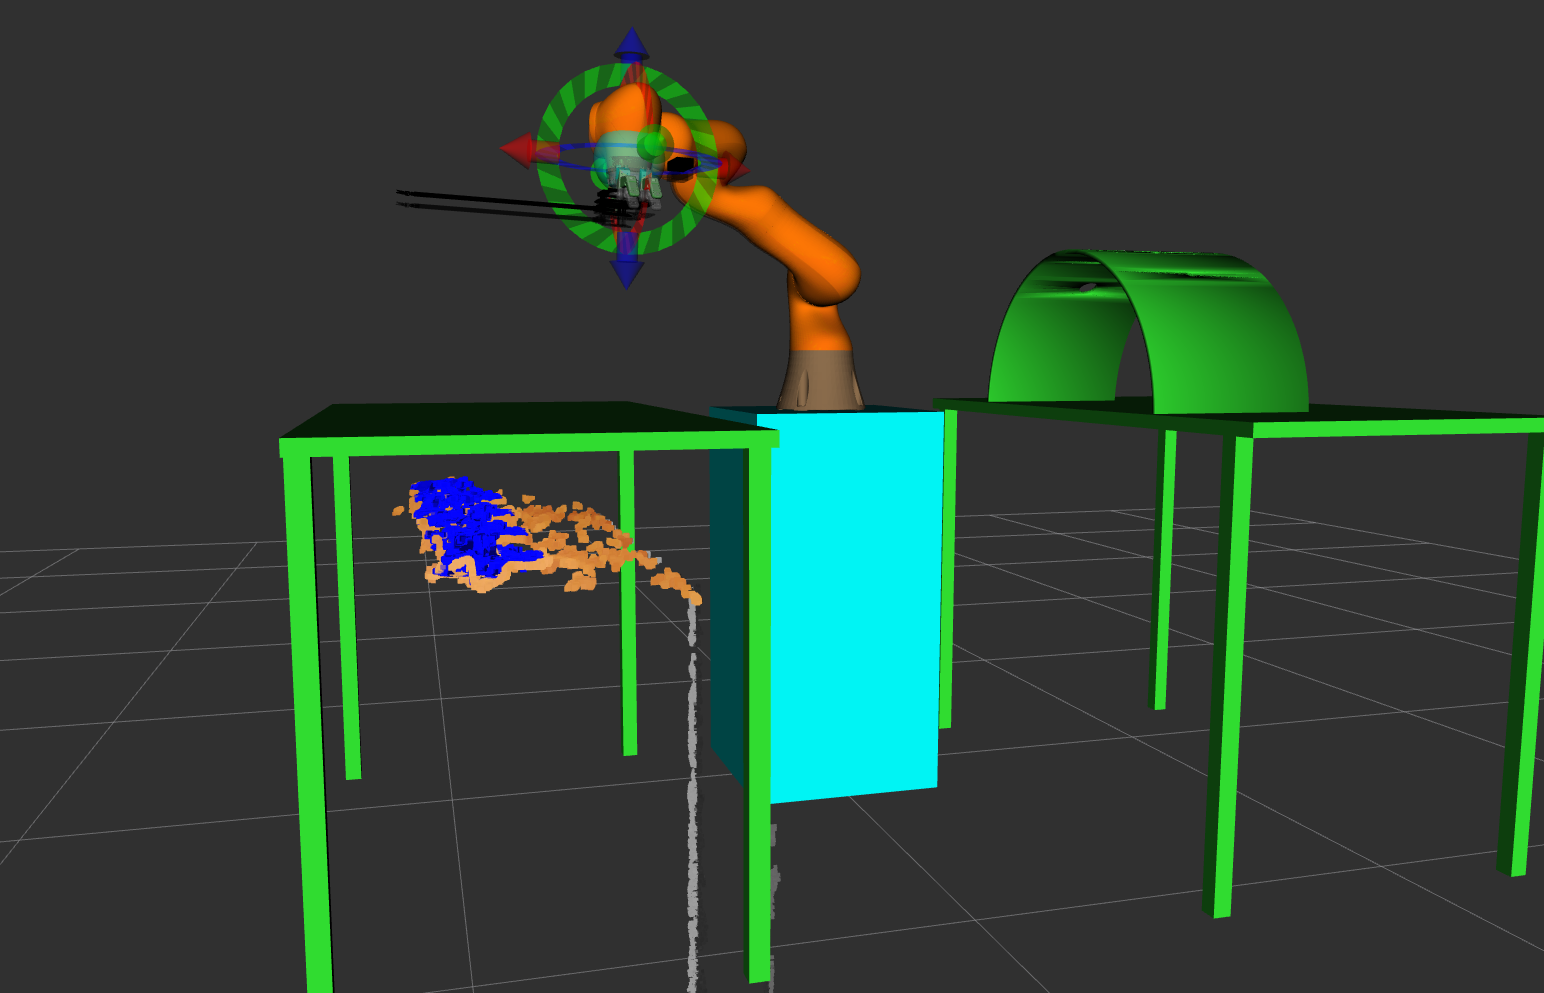
\includegraphics[width=12cm]{images/point_cloud.png}\\
  \caption{Point cloud of surgical tools, generated from the 2 cameras and visualized in RViz}
  \end{figure}
  \end{center}
\end{comment}

\section{Calculation of tool position and orientation}

In order for the gripper to grasp correctly the laparoscopic tool, it is required to calculate the tool's position and orientation in the pixel space 
which must then be converted with respect to the robot's workspace. From all the pixels that have been classified as part of the laparoscopic tool,  one can estimate the center of mass and two perpendicular vectors attached to that point that define the orientation. The center of mass is simply the average of the $(x,y)$ coordinates of all the tool's pixels
\begin{equation}
\left( \bar{x}, \bar{y} \right) = \left( \frac{1}{N}\sum_{i=1}^{N} x_i , \frac{1}{N}\sum_{i=1}^{N} y_i \right)
\end{equation}

The easiest way to calculate the center of mass is by calculating the average using the first moments of the contour points. However, since the contour is only using the boundary of the object and not it's area, this method is not very accurate. For a more accurate value for the center of mass, the pixels that are inside the detected object's contour are used. The simplest way to get the inside pixels of the tool is to loop over all the pixels and for each pixel check if it is inside the polygon. Pixel subsampling can be used to speed up the execution.

\begin{center}
\begin{figure}[htbp]
\centering
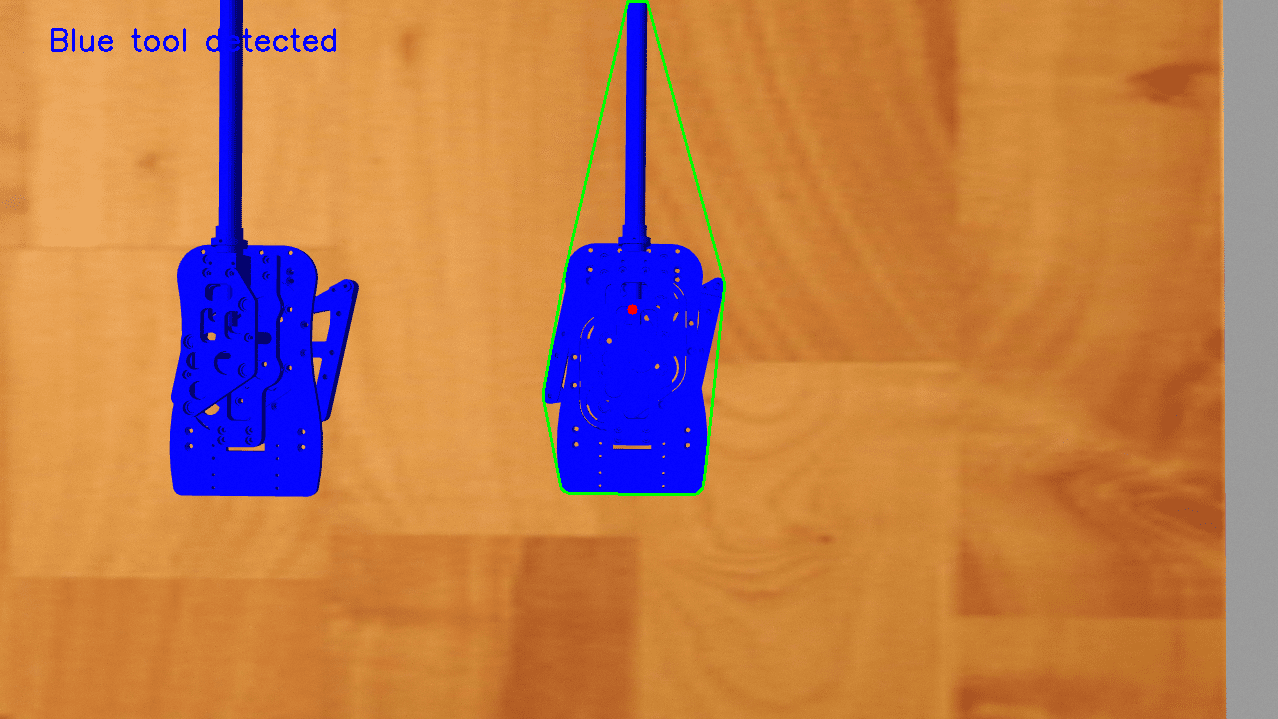
\includegraphics[width=0.7\textwidth]{images/opencv-tool-convex-hull.png}\\
\caption{Simple tool detection in simulation based on color, using OpenCV. The green polygon is the convex hull, and the red point is the estimated center of mass}
\end{figure}
\end{center}

This approach can be further optimized by accounting only those pixels inside the \textbf{Region of Interest} (ROI)  of the tool. ROI is a rectangular bounding box that fits exactly an object to be studied. Having already calculated the contour of the surgical tool and its convex hull we can easily calculate this bounding box. For this calculation we prefer to use the convex hull, because it often contains much less pixels than the contour. We iterate over all the pixels of the convex hull and we get the minimum and maximum x and y coordinates. The combination of these four values is the desired ROI. Since we now have access to the tool's ROI, we can iterate and sample the pixels inside it to get some of the pixels of the tool so that we can more accurately calculate its center of mass and orientation vectors. 

The two orientation vectors are the eigenvectors of the covariance matrix of the above pixels. Let $\mathbf{a},\mathbf{b}$ be the orientation vectors, 
then $\mathbf{a},\mathbf{b}$ are solutions of $
\mathbf{C} \mathbf{v} = λ \mathbf{v},~
$
where $\mathbf{C}$ is the covariance matrix given by

\begin{equation}
\label{eq:cov-matrix}
\mathbf{C} = \begin{bmatrix}
σ(x,x) & σ(x,y) \\
σ(y,x) & σ(y,y) \\
\end{bmatrix}
,~\mbox{and}~
\label{eq:cov-matrix-coeff}
σ(x,y) = \frac{1}{n-1} \sum_{i=1}^{N} ( x_i - \bar{x} )( y_i - \bar{y} ).
\end{equation}
\begin{center}
\begin{figure}[htbp]
\centering
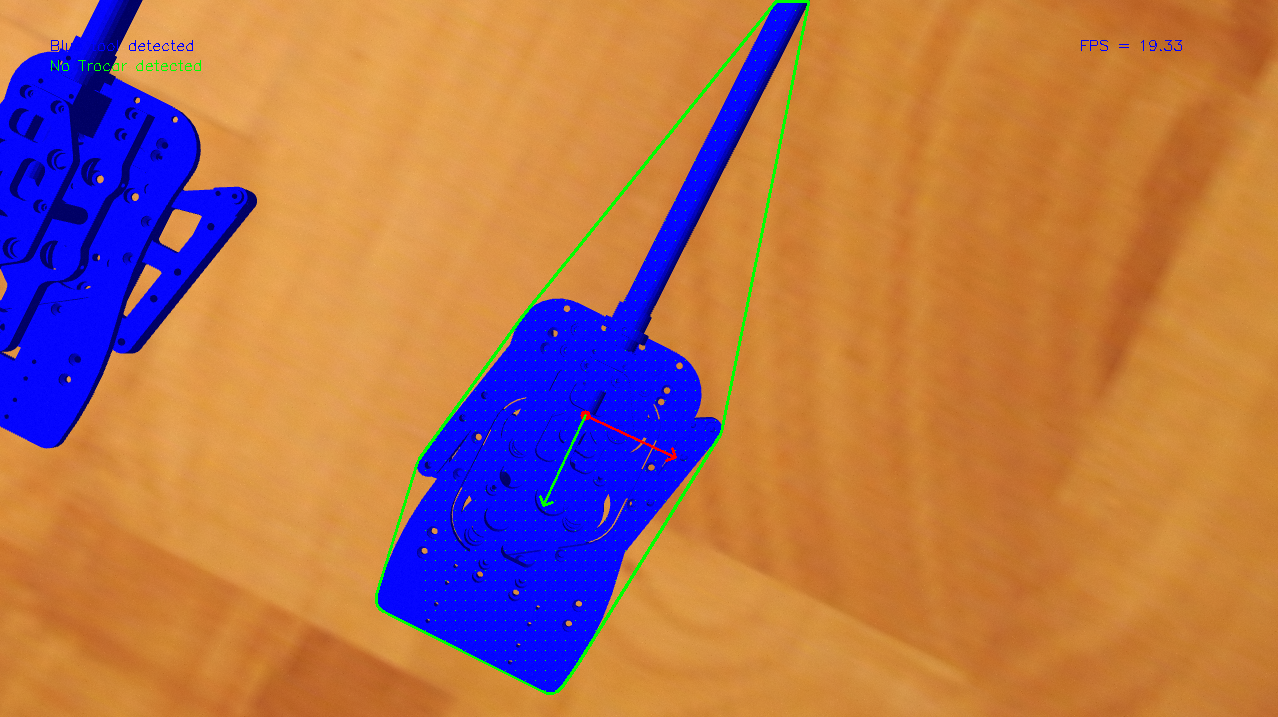
\includegraphics[width=0.7\textwidth]{images/tool-pose.png}\\
\caption{Estimation of tool's pose (position and orientation). The red dot is the center of mass and attached to that are the two orientation vectors of the tool. The green polygon is the convex hull of the tool 
and the white rectangle is its ROI.}
\end{figure}
\end{center}

\section{Calculation of grasping points}
%
The calculation of the candidate grasping points is a problem where we seek to find the points that lie on the contour of the detected object such that the gripper can make a good grasp of the object preferably with force closure. The adopted method is by using an expanding \textbf{growing circle}. This circle is initiated with a small radius and has at all times its center at the center of mass of the detected tool. At each step of the method the radius is incremented by a fixed amount and then we check if this circle has any intersection with the contour of the detected tool. If no intersection is found the method proceeds with a new radius. The method is terminated when at least three  intersections are found owing to the three finger-configuration of the hand.

the set of intersection points $\mathbb{G}$ is calculated from
\begin{equation}
\label{grasping-intersections}
\mathbb{G} = \underset{(x,y)}{\arg\max} I_1(x,y) \odot I_2(x,y).
\end{equation}
Given one binary image $I_1(x,y)$ which contains the contour of the detected tool (all white pixels are the contour) and one second binary image $I_2(x,y)$ which contains the growing circle, then the set of intersection points are the $(x, y)$ coordinates where the Hadamard product $I_1(x,y) \odot I_2(x,y)$ (element-wise product) of the two binary images is maximum.\\ 

Several times multiple pixels are returned from this method due to the "pixelated nature" of all curves. To filter all these pixels and get only one pixel for each intersection point we initialize a list of the final points with the first pixel found and then iterate over all of the other pixels. For each pixel we check if it has a Manhattan distance bigger than a threshold (e.g. 10) from the pixels that are already added in the list of the final pixels. If two pixels have a Manhattan distance bigger than a selected threshold then we consider them to be two different intersection points. The Manhattan distance of two points $\mathbf{p}_1=(x_1,y_1)$, ${\mathbf{p}_2=(x_2,y_2)}$ is $
d_1(\mathbf{p}_1, \mathbf{p}_2) = |x_1 - x_2| + |y_1 - y_2|
$.
\begin{center}
\begin{figure}[htbp]
\centering
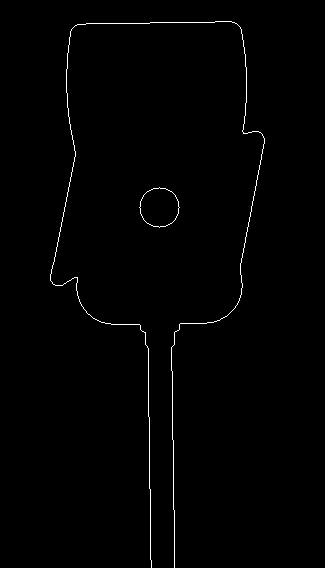
\includegraphics[width=0.2\textwidth]{images/grasp_points_1.png}
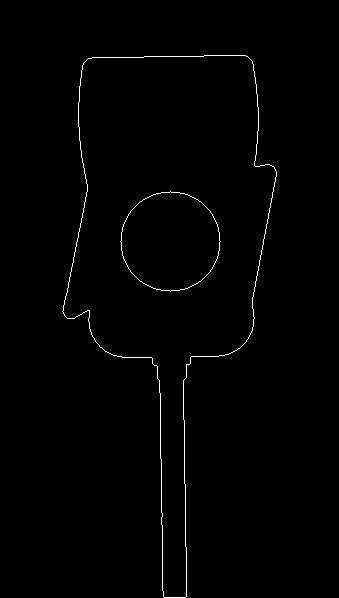
\includegraphics[width=0.2\textwidth]{images/grasp_points_2.png}
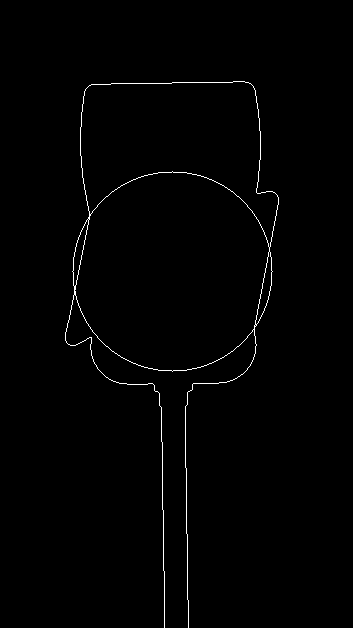
\includegraphics[width=0.2\textwidth]{images/grasp_points_3.png}\\
\caption{Finding candidate grasping points from the intersections of a growing circle and the contour of the detected surgical tool}
\end{figure}
\end{center}

%
\section{Trocar detection \& Estimation of fulcrum point}
%
The detection of the trocar is accomplished using a similar simple trivial detection algorithm as the one used in Section~\ref{laparoscopic-tool-detection}. The fulcrum point is assumed to be at the trocar's (cylindrical shape) center. 

\begin{center}
\begin{figure}[htbp]
\centering
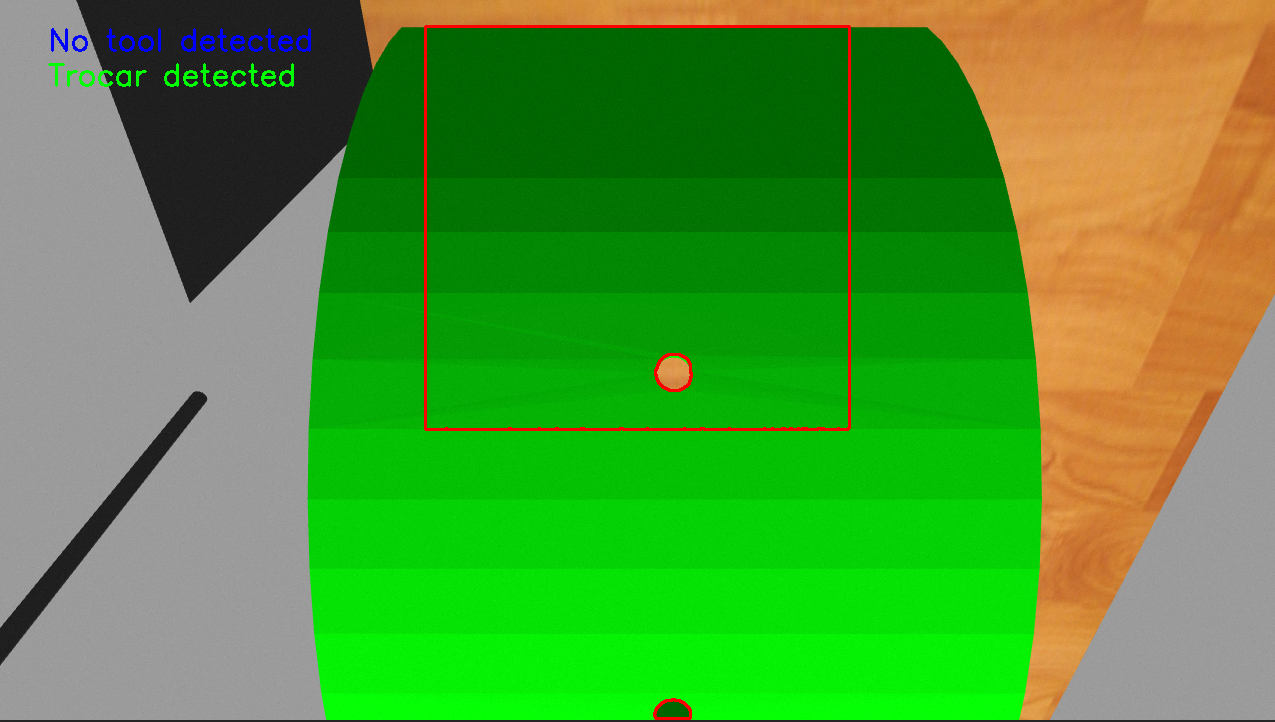
\includegraphics[width=0.7\textwidth]{images/opencv-trocar-detection.png}\\
\caption{Simple color-based trocar using OpenCV.}
\end{figure}
\end{center}
